\documentclass[conference]{IEEEtran}

\usepackage{amsmath,amssymb}
\usepackage{graphicx}
\usepackage{cite}
\usepackage{booktabs}
\usepackage{array}
\usepackage{siunitx}
\usepackage{xcolor}
\usepackage{tikz}
\usetikzlibrary{arrows.meta,positioning,calc}

\newcommand{\dummyfigure}[2]{%
\begin{figure}[!t]
\centering
\fbox{%
\begin{minipage}[c][1.45in][c]{0.92\linewidth}
\centering
\vspace{0.05in}
\textbf{Dummy Figure Placeholder}\\[0.5em]
\texttt{\detokenize{#1}}
\end{minipage}}
\caption{#2}
\label{fig:#1}
\end{figure}}

\begin{document}

\title{LQR and $H_\infty$ Control Comparison for a Two-Wheeled Self-Balancing Robot}

\author{\IEEEauthorblockN{First Author, Second Author}
\IEEEauthorblockA{Department of Mechanical Engineering\\
The University of Texas at Dallas\\
Richardson, TX, USA\\
Email: author@utdallas.edu}}

\maketitle

\begin{abstract}
This report compares linear quadratic regulator (LQR) and mixed-sensitivity $H_\infty$ controllers for a two-wheeled self-balancing robot. A one-input balancing formulation is used, where the same voltage command is distributed equally to the left and right motors. The controllers are evaluated using nominal initial-condition response, sinusoidal disturbance rejection, structured mass and height uncertainty, worst-case gain analysis, and Monte Carlo simulation over uncertain physical parameters. The LQR controller provides a simple full-state feedback baseline, while the $H_\infty$ controller explicitly shapes sensitivity, control effort, and high-frequency complementary sensitivity. The simulations show how the two methods trade nominal response, voltage usage, disturbance attenuation, and robustness to model uncertainty.
\end{abstract}

\begin{IEEEkeywords}
self-balancing robot, LQR, $H_\infty$ control, robust control, mixed sensitivity, Monte Carlo simulation
\end{IEEEkeywords}

\section{Introduction}
Two-wheeled self-balancing robots are nonlinear, underactuated systems whose upright equilibrium is open-loop unstable. Around the upright operating point, the balancing dynamics can be represented by a linear state-space model and stabilized using feedback control. Classical optimal control, such as LQR, is attractive because it gives a direct state-feedback law with transparent state and input penalties. However, performance can degrade under external disturbances and plant-parameter variations. Robust control methods such as $H_\infty$ synthesis can improve worst-case behavior by explicitly shaping closed-loop sensitivity and control effort.

This work studies a common-mode balancing input for a two-wheeled self-balancing robot. Four MATLAB scripts were used: the nominal one-input comparison, disturbance-rejection experiment, parametric-uncertainty experiment, and Monte Carlo simulation. The main objective is to compare LQR and $H_\infty$ controllers under increasingly uncertain operating conditions.

The main contributions are:
\begin{itemize}
\item A one-input common-mode balancing model is used so that LQR and $H_\infty$ controllers are compared under the same motor-voltage distribution.
\item Three uncertainty sources are considered: payload-mass variation, body-height variation, and external input disturbance.
\item The comparison includes nominal stabilization, disturbance rejection, robust performance, actuator voltage usage, and Monte Carlo validation.
\item The tradeoff between tight pitch regulation and actuator-safe robust behavior is explicitly evaluated.
\end{itemize}

\section{Robot Model}
The balancing subsystem is represented using the state vector
\begin{equation}
x=\begin{bmatrix}\theta & \psi & \dot{\theta} & \dot{\psi}\end{bmatrix}^T,
\end{equation}
where $\theta$ is the average wheel angle and $\psi$ is the body pitch angle. The nominal linear model used in the first two experiments is
\begin{equation}
\dot{x}=Ax+Bu,
\end{equation}
with
\begin{equation}
A=
\begin{bmatrix}
0 & 0 & 1 & 0\\
0 & 0 & 0 & 1\\
0 & 55.540 & -0.610 & 0.610\\
0 & 62.794 & -0.316 & 0.316
\end{bmatrix},
\end{equation}
and the original two-motor input matrix
\begin{equation}
B_2=
\begin{bmatrix}
0 & 0\\
0 & 0\\
9.385 & 9.385\\
-4.857 & -4.857
\end{bmatrix}.
\end{equation}
For balancing, the two motor voltages are commanded equally:
\begin{equation}
u_b=v_l+v_r,\qquad v_l=v_r=\frac{u_b}{2}.
\end{equation}
Therefore, the effective one-input model uses
\begin{equation}
B=B_2(:,1)=
\begin{bmatrix}
0 & 0 & 9.385 & -4.857
\end{bmatrix}^T.
\end{equation}
The output matrix is selected as $C=I_4$, so full-state feedback and full-state performance outputs are available.

\begin{table}[!t]
\caption{Nominal Physical Parameters Used in the Uncertainty Model}
\label{tab:physical_params}
\centering
\begin{tabular}{lcc}
\toprule
Parameter & Symbol & Nominal Value\\
\midrule
Payload/body mass & $M_0$ & $0.25$ kg\\
Robot height & $H_0$ & $0.17$ m\\
Wheel radius & $R$ & $0.0325$ m\\
Wheelbase width & $W$ & $0.192$ m\\
Body depth & $D$ & $0.082$ m\\
Gear ratio & $n$ & $30$\\
Motor resistance & $R_m$ & $2.9~\Omega$\\
Back-emf constant & $K_b$ & $0.024$\\
Torque constant & $K_t$ & $0.025$\\
\bottomrule
\end{tabular}
\end{table}

\section{Uncertainty Description and Robust Objective}
The presentation identifies three major uncertainty sources for the balancing problem. First, payload changes alter the total mass and shift the inertial properties. Second, height changes modify the center-of-mass location and therefore the gravitational torque about the wheel axis. Third, external disturbances act through the acceleration channels and represent pushes, floor irregularities, or unmodeled input effects.

The robust-control objective is therefore not only to stabilize the nominal plant. The closed-loop system should remain stable for the full modeled parameter range, keep pitch and wheel states bounded during disturbances, and satisfy practical actuator limits. In this project the motor-voltage limit is treated as
\begin{equation}
|v_l|,\ |v_r| \leq 24~\mathrm{V}.
\end{equation}
This actuator-safety requirement is important because a controller that gives excellent pitch regulation but demands unrealistic voltage is not physically implementable.

\begin{figure*}[!t]
\centering
\resizebox{0.92\textwidth}{!}{%
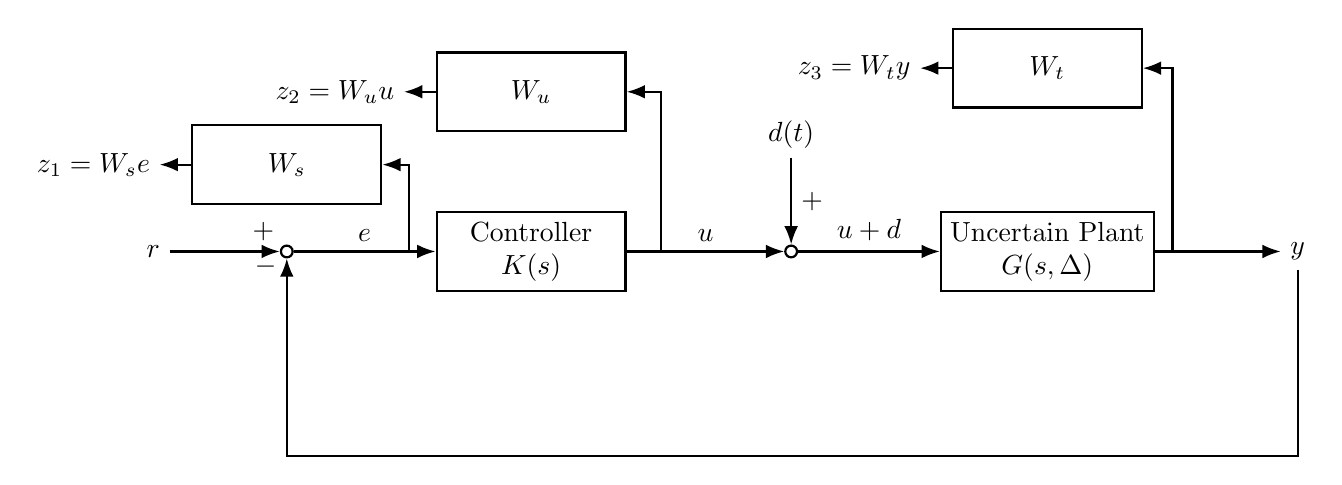
\begin{tikzpicture}[
    >=Latex,
    block/.style={draw, thick, rectangle, minimum height=1cm, minimum width=2.4cm, align=center},
    sum/.style={draw, circle, thick, inner sep=1.5pt},
    node distance=1.7cm
]
\node[sum] (sum_e) {};
\node[block, right=1.8cm of sum_e] (K) {Controller\\$K(s)$};
\node[sum, right=2.0cm of K] (sum_u) {};
\node[block, right=1.8cm of sum_u] (G) {Uncertain Plant\\$G(s,\Delta)$};
\node[right=1.6cm of G] (y) {$y$};
\node[left=1.4cm of sum_e] (r) {$r$};
\node[above=1.1cm of sum_u] (d) {$d(t)$};
\node[block, above=0.5cm of sum_e] (Ws) {$W_s$};
\node[block, above=1cm of K] (Wu) {$W_u$};
\node[block, above=1.3cm of G] (Wt) {$W_t$};
\node[left=0.4cm of Ws] (z1) {$z_1=W_s e$};
\node[left=0.4cm of Wu] (z2) {$z_2=W_u u$};
\node[left=0.4cm of Wt] (z3) {$z_3=W_t y$};

\draw[->, thick] (r) -- node[above,pos=0.85] {$+$} (sum_e);
\draw[->, thick] (sum_e) -- node[above] {$e$} (K);
\draw[->, thick] (K) -- node[above] {$u$} (sum_u);
\draw[->, thick] (sum_u) -- node[above] {$u+d$} (G);
\draw[->, thick] (G) -- (y);
\draw[->, thick] (d) -- node[right] {$+$} (sum_u);
\draw[->, thick] (y) |- ++(0,-2.6) -| node[pos=0.98,left] {$-$} (sum_e);
\draw[->, thick] ($(sum_e)!0.5!(K)$) |- (Ws);
\draw[->, thick] (Ws) -- (z1);
\draw[->, thick] ($(K)!0.5!(sum_u)$) |- (Wu);
\draw[->, thick] (Wu) -- (z2);
\draw[->, thick] ($(G)!0.5!(y)$) |- (Wt);
\draw[->, thick] (Wt) -- (z3);
\end{tikzpicture}}
\caption{Robust-control architecture for the mixed-sensitivity $H_\infty$ design.}
\label{fig:control-architecture}
\end{figure*}

\section{Controller Design}
\subsection{LQR Controller}
The LQR controller minimizes
\begin{equation}
J=\int_0^\infty \left(x^TQx+u^TRu\right)dt,
\end{equation}
and applies the state-feedback law
\begin{equation}
u_b=-K_{\mathrm{LQR}}x.
\end{equation}
The nominal simulations use
\begin{equation}
Q=\mathrm{diag}(10000,1,10000,1),
\end{equation}
with $R=200$ for the nominal initial-condition experiment and $R=500$ for the disturbance and uncertainty experiments. The large penalties on $\theta$ and $\dot{\theta}$ are used to regulate wheel motion while stabilizing body pitch.

LQR is useful as a nominal baseline, but it does not directly provide uncertainty guarantees, frequency-dependent performance shaping, or worst-case performance bounds. Actuator limits can only be handled indirectly by increasing $R$, which reduces control effort but may also reduce regulation performance.

\subsection{Mixed-Sensitivity $H_\infty$ Controller}
The $H_\infty$ controller is synthesized using MATLAB's \texttt{mixsyn} command. The design solves the mixed-sensitivity problem
\begin{equation}
\min_K \left\|
\begin{bmatrix}
W_sS\\
W_uKS\\
W_tT
\end{bmatrix}
\right\|_\infty,
\end{equation}
where
\begin{equation}
S=(I+GK)^{-1},\qquad T=GK(I+GK)^{-1}.
\end{equation}
The sensitivity weight has the form
\begin{equation}
W_{s,\mathrm{base}}(s)=\frac{s/M_s+\omega_b}{s+\omega_b A_s},
\end{equation}
with $M_s=3$, $A_s=0.15$, and $\omega_b=4$ rad/s. The weighting matrix penalizes pitch-related channels more strongly:
\begin{equation}
\begin{aligned}
W_s=\mathrm{blkdiag}(&0.01W_{s,\mathrm{base}},0.1W_{s,\mathrm{base}},\\
&0.005W_{s,\mathrm{base}},0.08W_{s,\mathrm{base}}).
\end{aligned}
\end{equation}
for Experiments 1 and 2. In Experiment 3, the pitch and pitch-rate weights are increased to $0.3W_s$ and $0.15W_s$, respectively. The control weight is selected from the motor-voltage limit:
\begin{equation}
W_u=\frac{1}{4u_{\max}},\qquad u_{\max}=24\ \mathrm{V},
\end{equation}
with a slightly different scaling in the uncertainty study. The complementary-sensitivity weight is
\begin{equation}
W_t=0.01\frac{s+\omega_t/M_t}{A_t s+\omega_t}I_4,
\end{equation}
where $M_t=3$, $A_t=5\times 10^{-2}$, and $\omega_t=50$ rad/s.

The weighted channels have the following interpretations. The $W_sS$ channel shapes disturbance rejection and low-frequency tracking behavior. The $W_uKS$ channel penalizes control effort and helps keep the motor voltage practical. The $W_tT$ channel limits high-frequency amplification and improves noise robustness. The achieved $H_\infty$ value $\gamma$ is used to evaluate how closely the weighted design specifications are satisfied.

\dummyfigure{mixed-sensitivity-bode}{Mixed-sensitivity frequency-response check for $W_sS$, $W_uKS$, and $W_tT$. Replace this placeholder with the weighted-channel Bode plot.}

\section{Simulation Experiments}
\subsection{Experiment 1: Nominal Initial-Condition Response}
The first experiment compares the nominal closed-loop response of LQR and $H_\infty$ control over 10 s with
\begin{equation}
x(0)=
\begin{bmatrix}
0 & 0.1 & 0.3 & 0.3
\end{bmatrix}^T.
\end{equation}
The response variables are average wheel angle, wheel angular velocity, body pitch angle, body pitch angular velocity, and left/right motor voltages.

\dummyfigure{exp1-nominal-response}{Nominal initial-condition response comparing LQR and $H_\infty$ controllers. Replace this placeholder with the six-subplot figure generated by \texttt{SELF\_BALANCING\_COMPARISON\_1INPUT.m}.}

\subsection{Experiment 2: Sinusoidal Disturbance Rejection}
The second experiment injects an external disturbance into the acceleration states:
\begin{equation}
\dot{x}=Ax+Bu+B_df(t),
\end{equation}
where
\begin{equation}
B_d=
\begin{bmatrix}
0 & 0 & 1 & 1
\end{bmatrix}^T,\qquad
f(t)=0.3\sin(t).
\end{equation}
The same initial condition as Experiment 1 is used. The LQR closed-loop system is simulated as
\begin{equation}
\dot{x}=(A-BK_{\mathrm{LQR}})x+B_df(t),
\end{equation}
while the $H_\infty$ controller is simulated using the augmented dynamic closed-loop model.

\dummyfigure{exp2-disturbance}{External sinusoidal disturbance $f(t)=0.3\sin(t)$. Replace this placeholder with the disturbance plot from Experiment 2.}

\dummyfigure{exp2-response}{Disturbance-rejection response comparing LQR and $H_\infty$ controllers. Replace this placeholder with the six-subplot response figure generated by \texttt{SELF\_BALANCING\_COMPARISON\_EXP2.m}.}

\subsection{Experiment 3: Parametric Uncertainty}
The third experiment evaluates robustness to physical parameter variation. The controllers are designed at the nominal values
\begin{equation}
M_0=0.25\ \mathrm{kg},\qquad H_0=0.17\ \mathrm{m},
\end{equation}
and then held fixed while the plant changes over
\begin{equation}
M\in[0.2,0.3]\ \mathrm{kg},\qquad H\in[0.14,0.20]\ \mathrm{m}.
\end{equation}
The script constructs the balancing model from physical parameters using the symbolic state-space function \texttt{twsbr\_symbolic\_ss}. The uncertain plant is modeled with \texttt{ureal} objects and analyzed using worst-case gain computations.

The presentation summary reports that both controllers remain robustly stable because the robust-stability margins are greater than one. However, the LQR design has a practical drawback: although it gives a stronger stability margin and tighter pitch stabilization, it can require approximately $67$ V in the uncertainty experiment, which exceeds the 24 V motor limit. The $H_\infty$ controller has a smaller robust margin and allows larger transient motion, but it remains actuator-safe across the modeled mass and height variations. The reported $H_\infty$ synthesis value is approximately $\gamma=2$, meaning the strict mixed-sensitivity target $\gamma<1$ is not fully achieved, but the closed-loop system remains robustly stable.

\dummyfigure{exp3-endpoint}{Endpoint parameter-change response for nominal, mass-change, height-change, and combined-change cases. Replace this placeholder with the Experiment 3 pitch, wheel-angle, or motor-voltage figure.}

\dummyfigure{exp3-robust-margin}{Robustness and worst-case gain comparison between LQR and $H_\infty$. Replace this placeholder with the bar plot generated in the uncertainty analysis.}

\subsection{Monte Carlo Uncertainty Simulation}
The Monte Carlo script samples uncertain mass and height values and simulates both controllers for each sample. For each run, the following metrics are recorded:
\begin{equation}
\max_t|\psi(t)|,\qquad \max_t|v_l(t)|,
\end{equation}
along with closed-loop stability. The script uses $N_{\mathrm{MC}}=10000$ samples and overlays nominal pitch response on the sampled trajectories.

\dummyfigure{mc-pitch}{Monte Carlo pitch-angle responses for LQR and $H_\infty$. Replace this placeholder with the figure generated by \texttt{SELF\_BALANCING\_MONTE\_CARLO\_SIM.m}.}

\dummyfigure{mc-metrics}{Monte Carlo histograms and scatter plots for pitch peak and voltage peak metrics. Replace this placeholder with the Monte Carlo metrics figure.}

\section{Performance Metrics}
The MATLAB scripts print peak pitch angle, peak control input, peak motor voltage, $H_\infty$ synthesis $\gamma$, worst-case gains, and Monte Carlo stability counts. Table~\ref{tab:nominal_metrics} and Table~\ref{tab:robust_metrics} provide report-ready locations for those values.

\begin{table}[!t]
\caption{Nominal and Disturbance-Rejection Metrics}
\label{tab:nominal_metrics}
\centering
\begin{tabular}{lcc}
\toprule
Metric & LQR & $H_\infty$\\
\midrule
Experiment 1 max $|\psi|$ (rad) & TBD & TBD\\
Experiment 1 max $|u_b|$ (V) & TBD & TBD\\
Experiment 1 max $|v_l|$ (V) & TBD & TBD\\
Experiment 2 max $|\theta|$ (rad) & TBD & TBD\\
Experiment 2 max $|\psi|$ (rad) & TBD & TBD\\
Experiment 2 max $|v_l|$ (V) & TBD & TBD\\
\bottomrule
\end{tabular}
\end{table}

\begin{table}[!t]
\caption{Robustness and Monte Carlo Metrics}
\label{tab:robust_metrics}
\centering
\begin{tabular}{lcc}
\toprule
Metric & LQR & $H_\infty$\\
\midrule
Worst-case gain lower bound & TBD & TBD\\
Worst-case gain upper bound & TBD & TBD\\
Stable Monte Carlo samples & TBD & TBD\\
Monte Carlo max $|\psi|$ (rad) & TBD & TBD\\
Monte Carlo mean max $|\psi|$ (rad) & TBD & TBD\\
Monte Carlo max $|v_l|$ (V) & TBD & TBD\\
\bottomrule
\end{tabular}
\end{table}

\begin{table}[!t]
\caption{Qualitative Comparison from Simulation Study}
\label{tab:qualitative}
\centering
\begin{tabular}{p{0.31\linewidth}p{0.25\linewidth}p{0.25\linewidth}}
\toprule
Criterion & LQR & $H_\infty$\\
\midrule
Controller type & Static state feedback & Dynamic robust controller\\
Nominal pitch regulation & Tighter & More conservative\\
Frequency shaping & Not explicit & Explicit through weights\\
Uncertainty guarantee & Not direct & Designed for worst-case behavior\\
Motor-voltage behavior & Can be aggressive & Actuator-aware through $W_u$\\
Robust design tradeoff & Higher regulation effort & Safer voltage usage\\
\bottomrule
\end{tabular}
\end{table}

\section{Discussion}
The LQR controller gives a low-order state-feedback law and is straightforward to tune through $Q$ and $R$. Its behavior depends strongly on the nominal model and the selected state penalties. The $H_\infty$ controller is dynamic and higher order, but it directly accounts for sensitivity, control effort, and high-frequency response during synthesis. This structure is useful for disturbance rejection and uncertainty studies because the controller is designed around worst-case closed-loop transfer behavior.

The disturbance experiment tests the controllers under a persistent sinusoidal input applied through the acceleration states. A controller with lower sensitivity in the disturbance frequency range should reduce the peak pitch response. The uncertainty experiment evaluates whether the nominally designed controllers remain effective as payload mass and robot height change. The worst-case gain and Monte Carlo simulations provide complementary evidence: worst-case analysis searches for adverse parameter combinations, while Monte Carlo simulation estimates behavior over many sampled plants.

The key engineering tradeoff is between regulation aggressiveness and implementability. LQR can be tuned to produce strong nominal stabilization and smaller pitch transients, but this may require large motor voltages when the plant parameters shift. The $H_\infty$ controller sacrifices some transient regulation to reduce worst-case amplification and control demand. For a real robot, this is often the more practical choice because motor saturation can destabilize an otherwise successful simulation controller.

\section{Conclusion}
This report presented an IEEE conference-style comparison of LQR and mixed-sensitivity $H_\infty$ control for a two-wheeled self-balancing robot. The one-input common-mode balancing model was used to distribute voltage commands equally to both motors. Simulations were organized into nominal initial-condition response, sinusoidal disturbance rejection, structured mass/height uncertainty, and Monte Carlo sampling. The LQR controller is simpler and easier to implement, while the $H_\infty$ controller provides an explicit framework for shaping robustness and disturbance attenuation. The final numerical comparison should be completed by inserting the MATLAB-generated metrics and replacing the dummy figure placeholders with exported simulation plots.

\begin{thebibliography}{1}

\bibitem{zhou}
K. Zhou, J. C. Doyle, and K. Glover, \emph{Robust and Optimal Control}. Upper Saddle River, NJ, USA: Prentice Hall, 1996.

\bibitem{ogata}
K. Ogata, \emph{Modern Control Engineering}, 5th ed. Upper Saddle River, NJ, USA: Prentice Hall, 2010.

\bibitem{mathworks}
MathWorks, ``Robust Control Toolbox User's Guide,'' Natick, MA, USA.

\bibitem{twsbr}
F. Grasser, A. D'Arrigo, S. Colombi, and A. C. Rufer, ``JOE: A mobile, inverted pendulum,'' \emph{IEEE Transactions on Industrial Electronics}, vol. 49, no. 1, pp. 107--114, Feb. 2002.

\bibitem{spong}
M. W. Spong, S. Hutchinson, and M. Vidyasagar, \emph{Robot Modeling and Control}. Hoboken, NJ, USA: Wiley, 2006.

\bibitem{doyle}
J. C. Doyle, B. A. Francis, and A. R. Tannenbaum, \emph{Feedback Control Theory}. New York, NY, USA: Macmillan, 1992.

\bibitem{kwakernaak}
H. Kwakernaak and R. Sivan, \emph{Linear Optimal Control Systems}. New York, NY, USA: Wiley, 1972.

\end{thebibliography}

\end{document}
